\chapter[CredsRead]{CredsRead\raisebox{.3\baselineskip}{\normalsize\footnotemark}}
\footnotetext{\url{https://github.com/oliviercailloux/creds-read}}

CredsRead, pour Credentials Read, gère comme son nom l'indique la lecture des identifiants d'un utilisateur.

\section{Diagramme de classe}
Le diagramme de classe permet de avoir une idée précise du code que l'on veut écrire. Papyrus est un outil permettant de réaliser ce genre de diagramme. Son interface intuitive facilite la rédaction d'un diagramme UML(le langage standard des diagrammes de classe) lisible et rigoureux. 

\begin{figure}[!h]
    \begin{center}
    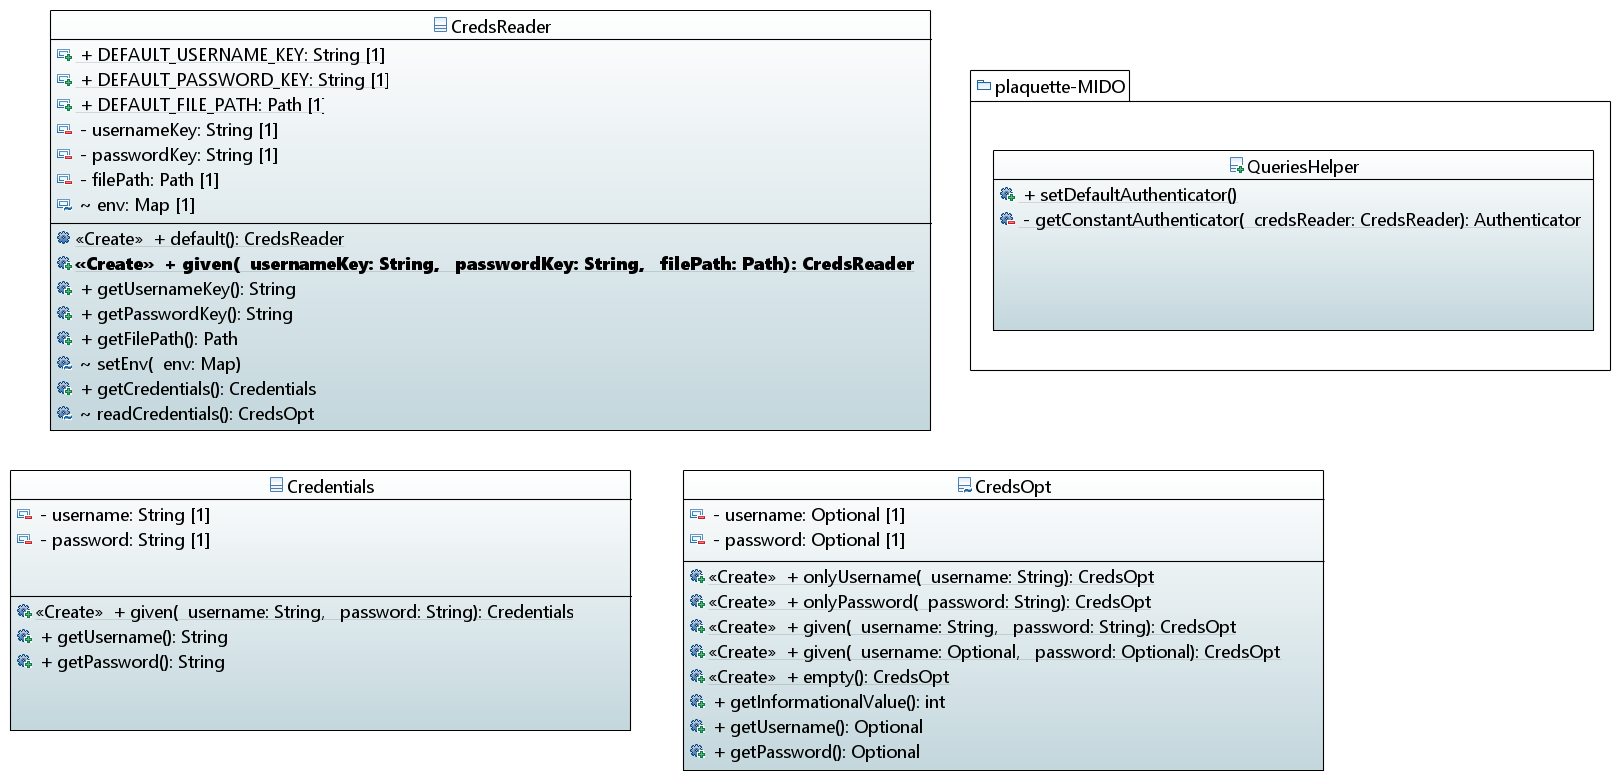
\includegraphics[width=\textwidth]{assets/doc.png}
    \end{center}
    \caption{Diagramme de classe du projet CredsRead}
\end{figure}